\documentclass[11pt]{hmcpset}
\usepackage[margin=1in]{geometry}
\usepackage{amsmath,amssymb,enumerate,graphicx,url}

\newcommand{\ket}[1]{|#1\rangle}
\newcommand{\bra}[1]{\langle #1|}
\newcommand{\braket}[2]{\langle #1|#2\rangle}
\newcommand{\braketop}[3]{\langle #1| #2 | #3 \rangle}
\newcommand{\normsq}[1]{\left|#1\right|^2}
\newcommand{\prob}[2]{\normsq{\braket{#1}{#2}}}
\newcommand{\avg}[1]{\langle #1 \rangle}


\usepackage{xcolor}
\usepackage{listings}

\definecolor{mGreen}{rgb}{0,0.6,0}
\definecolor{mGray}{rgb}{0.5,0.5,0.5}
\definecolor{mPurple}{rgb}{0.58,0,0.82}
\definecolor{backgroundColour}{rgb}{0.95,0.95,0.92}

\lstdefinestyle{Python}
{
	language=Python,
	backgroundcolor=\color{backgroundColour},   
	commentstyle=\color{mGreen},
	keywordstyle=\color{magenta},
	numberstyle=\tiny\color{mGray},
	stringstyle=\color{mPurple},
	basicstyle=\footnotesize\ttfamily,
	breakatwhitespace=false,         
	breaklines=true,                 
	captionpos=b,                    
	keepspaces=true,                 
	%numbers=left,                    
	numbersep=5pt,                  
	showspaces=false,                
	showstringspaces=false,
	showtabs=false,                  
	tabsize=3
}



\name{}
\class{PHYS134}
\assignment{Homework/Project 4}
\duedate{2021-03-05 (before spring break)}

\begin{document}
\problemlist{Knife Fit; Steck Section 6.6}




%===========================================================
%\begin{problem}[Steck 6.1 (5\,pts)]
%	A common technique in the laboratory for measuring the beam waist parameter of a Gaussian beam 	is illustrated in the diagram. A Gaussian beam is incident on an optical power meter, which registers 	the total power of the incident beam. A knife edge can be translated in the transverse direction to 	block part of the beam (i.e., if the position of the knife edge is $x_\mathrm{knife}$, then the parts of the beam with $x < x_\mathrm{knife}$ is blocked from reaching the power meter). The ``10-90'' rule is to measure the knife edge position $x_{10\%}$ where the power meter reads 10\% of the total beam power, and then the position	$x_{90\%}$ where the power meter reads 90\% of the total beam power. Then the beam radius $w(z)$ at the knife-edge location z along the beam is given by
%	\[
%	w(z) = \alpha \left| x_{10\%} - x_{90\%} \right|,
%	\]
%	where $\alpha$ is some constant factor. Calculate the numerical value of $\alpha$.
%	
%	\textit{Jason's Note:} The figure below shows this setup for the special case where the waist $w_0$ is measured. Justify briefly why the measurement at some non-zero $z$ position gives you $w(z)$.
%	
%	\begin{center}
%		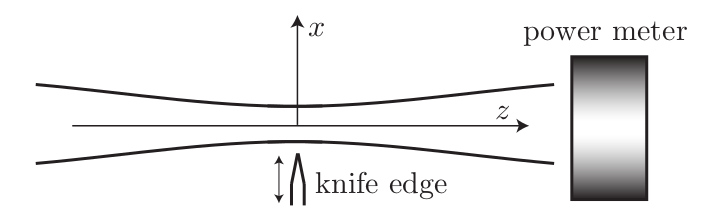
\includegraphics[width=0.6\textwidth]{knife_edge_beam}
%	\end{center}
%\end{problem}
%
%\begin{solution}
%	
%	\vfill
%	
%\end{solution}
%\pagebreak




%===========================================================
\begin{problem}[Gaussian Fit to Beam (10\,pts)]
	Watch the video \texttt{Lab4bHeNeLaserCavity\_BeamProfile.mov} in the OpticsLab2021 Google Drive. Direct link: \url{https://drive.google.com/file/d/1is-JH-bAUDqZ9K6NLT1b2jNuAYyUjfuz/view?usp=sharing} \\
	
	Download the data that I took and recorded in the CSV file:
	
	\texttt{Lab4bHeNeLaserCavity\_BeamProfile\_Data.csv}. \\
	
	From the section problem, you should have an expression for the power that makes it past a knife in various positions. Do a fit to determine $w$ at the location of the knife edge along with any other ``nuisance parameters'' like an arbitrary position offset and power-meter offset. It will be your first non-linear fit and your first with more than two parameters. Non-linear fits often require an initial guess for the parameters, which you can specify as the \texttt{p0} parameter of \texttt{curve\_fit}. \\
	
	Be sure to show Residuals, Normalized Residuals, and calculate $\chi^2$, $\chi^2$ per degree of freedom taking into account the number of fit parameters, and the probability-to-exceed (PTE). \\
	
	When I did the fit, it looked good, but had awful $\chi^2$ and PTE values. Unless I screwed up, this tells me that my errors are not statistical, but systematic. Perhaps the razor wasn't vertical or completely straight; perhaps there was a lot of scattered light that changed in a repeatable way as I moved the laser; or perhaps the beam wasn't Gaussian at the level of accuracy that the micrometer and power meter can measure. \\
	
	Assume that I was close enough to the focus of the laser to treat $w$ as $w_0$. Calculate $z_0$ from this. Based on the video, was that a reasonable assumption to make?
\end{problem}

\begin{solution}
	\vfill
\end{solution}
\pagebreak




%===========================================================
%\begin{problem}[Gaussian Beam Propagation (5\,pts)]
%Use camera to capture beam size at several places, meters away from HeNe. One location also had 10-90 rule applied to work out pixel scale. Check that the beam size as a function of distance away from the laser is consistent with the Gaussian Beam propagation. Where is the origin? (Closer to the laser's front or closer to its center?) Calculate the depth-of-focus $z_0$ parameter? Calculate full-angle divergence in the far field?
%\end{problem}
%
%\begin{solution}
%\vfill
%\end{solution}
%\pagebreak



%===========================================================
\begin{problem}[Steck Section 6.6 (10\,pts)]
	For a HeNe laser with $w_0=0.5$\,mm, reproduce the intensity plots in the figures in section 6.6 along with colorized phase plots for
	\begin{itemize}
		\item Hermite-Gaussian modes (p104)
		\item Doughnut mode (page 105) and 
		\item Laguerre-Gaussian Modes for a few of your favorite $l$ and $m$ (page 105 not shown)
	\end{itemize}
	Ignore overall constant amplitudes---just scale things so that the plots look reasonable. You will need to choose reasonable parameters for $z$ and the size of your screen. Be sure to indicate units on your plot and the location $z$ in the title along with what you're plotting. I'll just be looking at your plots and their titles, not code or comments. \\
	
	\textit{Motivation:} Watch the video \texttt{Lab4aHeNeLaserCavity\_SpatialModes.mp4} Direct link: \url{https://drive.google.com/file/d/18ADlwecpoW-YqBNyISwMZ7UVTrAuQgjF/view?usp=sharing} \\
	
	\textit{Hint:} You can use \texttt{Plane Waves Real and Complex.ipynb} as a template and just copy the \texttt{colorize} function directly to help plot complex functions.
\end{problem}

\begin{solution}
	\vfill
\end{solution}
\pagebreak



%===========================================================
%\begin{problem}[Steck 6.13 (5\,pts)]
%	Consider two monochromatic, Gaussian beams: a ``red'' beam of frequency $\omega$, and a ``blue'' beam
%	of frequency $2\omega$. Both have identical transverse intensity profiles at their respective foci, which both occur at the origin. Describe completely how the geometries (both near- and far-field) of the two fields differ. [Draw a picture of the two overlapping beams in two different colors and try to be somehwat accurate about what might be 2$\times$ or 4$\times$ as big: far-field diverge angles, depth-of-focus parameters $z_0$ for each beam, etc.]
%\end{problem}
%
%\begin{solution}
%	\vfill
%\end{solution}
%\pagebreak




%===========================================================
%\begin{problem}[Steck 6.14 (5\,pts)]
%	A monochromatic Gaussian beam (with beam waist parameter $w_0$) is focused onto a thin, nonlinear
%	optical element, whose effect on the (real) incident field is $E_\mathrm{out} = \alpha (E_\mathrm{in})^2$,
%	where $\alpha$ is some constant. Show that if the optical frequency of the input beam is $\omega$, the output field has a component with optical frequency $2\omega$. Describe completely how the geometry (both near- and
%	far-field) of the $2\omega$ output field differs from the input field.
%	
%	\textit{Hint:} The nonlinear optical element only acts at $z = 0$, so consider what the field looks like there.
%	
%	\textit{Jason's Hint:} Understand problem 6.13 first. In the lab, we create pairs of quantum-mechanically entangled photons using a non-linear crystal that acts a bit like this.
%\end{problem}
%
%\begin{solution}
%	\vfill
%\end{solution}
%\pagebreak


%===========================================================
%\begin{problem}[Couple HeHe into Cavity (5\,pts)]
%	Pick a lens to couple the HeNe laser in the above problems into a cavity with .... Where should the lens go and what should its focal length be to turn the laser into the beam we care about?
%\end{problem}
%\begin{solution}
%	\vfill
%\end{solution}
%\pagebreak


%===========================================================
%\begin{problem}[Couple 405\,nm Laser into crystal and 810\,nm light out (5\,pts)]
%	Given 50\,mm lens for 405\,nm, what is the spot size at the crystal. Measure with a razor blade on the mount in each direction. Couple out 810\,nm with 40\,mm lens. Mode match eventually to fiber. What's its deal?
%\end{problem}
%\begin{solution}
%	\vfill
%\end{solution}
%\pagebreak



\end{document}
